\documentclass[11pt]{article}
\usepackage[T1]{fontenc}
\usepackage[utf8]{inputenc}
\usepackage{lmodern,microtype}
\usepackage[margin=0.88in]{geometry}
\usepackage{amsmath,amssymb,graphicx,booktabs,longtable,array}
\usepackage[font=small,labelfont=bf]{caption}
\usepackage[numbers,sort&compress]{natbib}
\usepackage[hidelinks]{hyperref}
\usepackage{tikz}
\usetikzlibrary{arrows.meta,positioning}
\hypersetup{pdfauthor={Suneet Dungrani},pdfsubject={Preprint; not peer reviewed},pdfkeywords={robot design,verification,simulation,manufacturing,evidence}}
\setlength{\parskip}{3pt}
\setlength{\parindent}{1em}
\setlength{\emergencystretch}{2em}
\newcommand{\status}[1]{\textsf{#1}}
\newcommand{\EOneAggregateCad}{0.166667}
\newcommand{\EOneAggregateCadHigh}{0.333333}
\newcommand{\EOneAggregateCadHighRounded}{0.333}
\newcommand{\EOneAggregateCadLow}{0.000000}
\newcommand{\EOneAggregateCadRounded}{0.167}
\newcommand{\EOneAggregatePass}{17}
\newcommand{\EOneCadPass}{14}
\newcommand{\EOnePrimary}{0.055556}
\newcommand{\EOnePrimaryHigh}{0.166667}
\newcommand{\EOnePrimaryHighRounded}{0.167}
\newcommand{\EOnePrimaryLow}{0.000000}
\newcommand{\EOnePrimaryRounded}{0.056}
\newcommand{\EOneStructuredCad}{0.222222}
\newcommand{\EOneStructuredCadHigh}{0.444444}
\newcommand{\EOneStructuredCadHighRounded}{0.444}
\newcommand{\EOneStructuredCadLow}{0.000000}
\newcommand{\EOneStructuredCadRounded}{0.222}
\newcommand{\EOneStructuredPass}{18}
\newcommand{\EThreeCombined}{1.994444}
\newcommand{\EThreeInteraction}{0.161111}
\newcommand{\EThreeMechanical}{0.355556}
\newcommand{\EThreeScheduling}{1.477778}
\newcommand{\ETwoFastOriginal}{91}
\newcommand{\ETwoFastRevised}{98}
\newcommand{\ETwoReferenceOriginal}{96}
\newcommand{\ETwoReferenceRevised}{100}
\newcommand{\GantryBaselinePass}{59}
\newcommand{\GantryBaselinePrecise}{21.760000000}
\newcommand{\GantryBaselineTime}{21.760}
\newcommand{\GantryContinuous}{7.473751191}
\newcommand{\GantryDifference}{-0.01}
\newcommand{\GantryHigh}{0.04}
\newcommand{\GantryLow}{-0.07}
\newcommand{\GantryOptimisedPass}{58}
\newcommand{\GantryOptimisedPrecise}{7.473960844}
\newcommand{\GantryOptimisedTime}{7.474}
\newcommand{\TokensAggregate}{5,943,334}
\newcommand{\TokensCad}{4,369,703}
\newcommand{\TokensStructured}{6,638,533}

\newcommand{\authorblock}{Suneet Dungrani\\Independent Researcher\\\small\href{mailto:suneetdungrani@utexas.edu}{suneetdungrani@utexas.edu}}

\newcommand{\PlacementPairSentence}{The fast profile has 90 both-pass, 8 revised-only, 1 original-only and 1 both-fail draws.}

\hypersetup{pdftitle={FORGE: Evidence-Linked Robot Design, Verification, and Manufacturing Evaluation}}
\title{FORGE: Evidence-Linked Robot Design, Verification, and Manufacturing Evaluation}
\author{\authorblock}
\date{November 19, 2026\\\small Preprint \textperiodcentered{} Not peer reviewed}
\begin{document}
\maketitle
\begin{abstract}
A generated robot assembly can be editable and visually plausible while its engineering requirements remain unresolved. Forge associates design revisions with protected checks, simulated operation and a finite production model, retaining the scope and identity of each supporting observation. Controlled studies examine the consequences of this separation. In a 54-episode template-based repair study, CAD diagnostics, aggregate feedback and structured witnesses produced \EOneCadPass{}, \EOneAggregatePass{} and \EOneStructuredPass{} held-out passes out of 18 episodes per condition. Ten episodes changed from an initially failing build-valid candidate to a passing selected candidate. The primary structured-minus-aggregate difference was \EOnePrimaryRounded{}, with a nine-task cluster bootstrap interval of [0, \EOnePrimaryHighRounded{}], leaving a richer-feedback benefit unestablished. Previously collected paired simulations gave \ETwoReferenceOriginal{}/100 original-fixture and \ETwoReferenceRevised{}/100 revised-fixture passes, with numerically fragile near-threshold decisions. A separate fixed-path conic speed profile reduced planned gantry duration from \GantryBaselineTime{} to \GantryOptimisedTime{} s while successful simulated transfers changed from \GantryBaselinePass{}/100 to \GantryOptimisedPass{}/100. Production-model comparisons attributed a larger reference-cell gain to dispatch than to the fixture change. These results support an inspectable connection between revisions, bounded evaluations and downstream calculations; they do not establish physical robot reliability or general design-repair efficacy.
\end{abstract}
\noindent\textbf{Keywords:} robot design; scoped verification; design repair; contact simulation; time parameterization; discrete-event production.

\section{Introduction}
Robot design tools increasingly combine language-based specification, parametric geometry and simulation. These capabilities leave a practical question: what conclusion is justified for a particular assembly after its geometry, requirements or controller changes? A successful model export answers whether a representation was produced. A collision-free sample answers a narrower geometric question. A completed simulated operation concerns a modeled plant and disturbance draw. None of these observations, alone, establishes that a manufactured robot will satisfy its task.

Forge organizes these observations around the revision being evaluated. An input revision identifies the requirements; a candidate revision identifies editable geometry; protected checks produce measurements and witnesses; operation trials supply conditional outcomes; a production model consumes a separately specified operation envelope. The resulting evidence can be inspected and superseded without overwriting the observations that supported an earlier conclusion. The technical concern is the relationship among these layers, including cases where their conclusions disagree.

This paper evaluates that relationship through five studies. A known-answer geometry study examines acceptance, rejection and abstention under explicit checker scopes. A budget-matched agent study tests whether more detailed development feedback changes success on sealed evaluation draws. A fixture case study connects a coupled geometric change to paired placement outcomes. A gantry study applies established convex speed optimization to a fixed path and then checks complete simulated transfers. Finally, a four-cell production model separates mechanical, dispatch and interaction contrasts. Product journeys establish implemented evidence navigation, without serving as additional experimental samples.

The principal observation is that successful computation at one layer can coexist with unresolved engineering at the next. Design repairs occurred, but the primary feedback contrast remains inconclusive. A faster planned gantry motion did not improve transfer success. The production model assigned more of its reference-cell gain to dispatch than to fixture replacement. A feature-local wall check accepted cases while its whole-part projection correctly remained undecided. These are useful distinctions for engineering decisions, provided their scope remains attached to the result.

\begin{figure}[tb]
\centering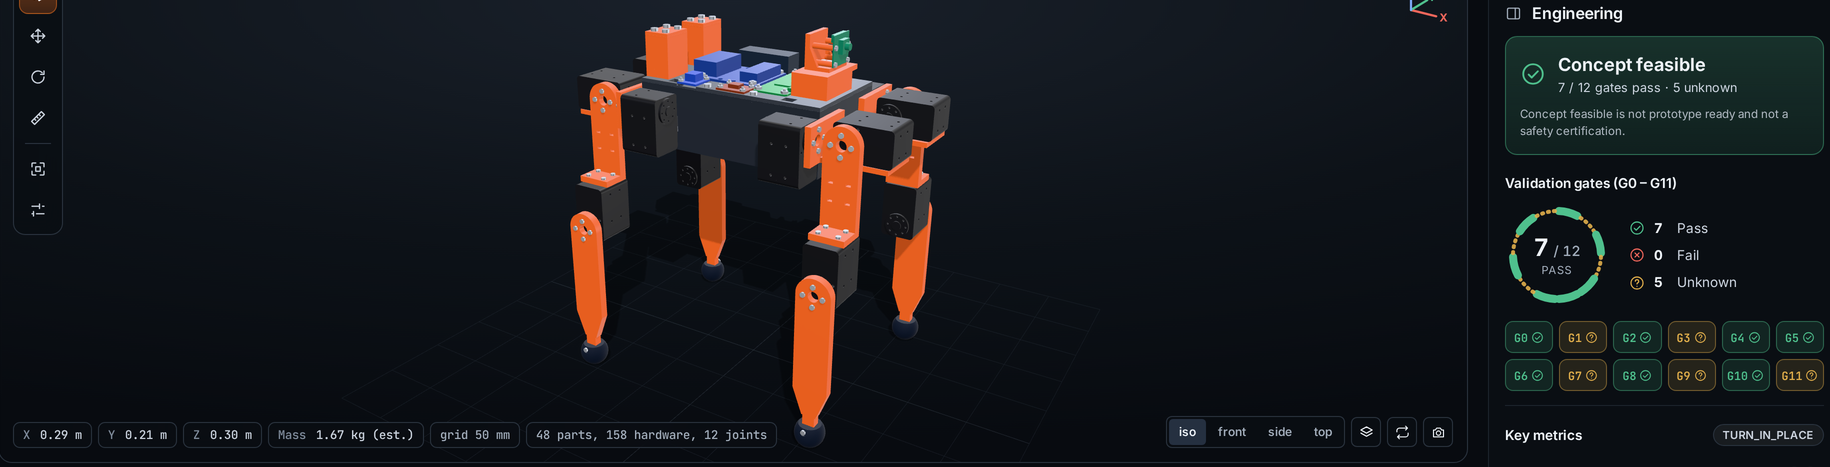
\includegraphics[width=\linewidth]{figures/native_quadruped.png}
\caption{Cropped native design-workspace capture of the separate inspection-quadruped project, shown as a design under test. Seven of twelve gates pass and five remain unknown. This interface view demonstrates assembly inspection and scoped evidence presentation; it supplies no fixture-study measurements or physical validation.}
\label{fig:native}
\end{figure}

\section{Context and related work}
Test-driven CAD generation and physics feedback predate this system. SPADA combines parametric assembly generation with deterministic evaluators, generated tests and repair diagnostics~\cite{zheng2026spada}. Physics-in-the-Loop couples CadQuery design with structural analysis and deterministic evaluation, including feedback ablations~\cite{berger2026physics}. Those methods make a generic compile--check--repair loop an inappropriate novelty claim. Forge's experiments instead concern revision-bound evidence across several representations and the measured behavior of distinct feedback conditions in a constrained robot task.

Parametric CAD Bench v3 evaluates artifact-level geometry and specification reward; CADWorld evaluates long-horizon computer use with persistent CAD artifacts and executable checks, including manufacturing and finite-element tasks~\cite{chen2026parametriccadbench,dong2026cadworld}. Their tasks, interfaces, budgets and reward definitions differ from the binary held-out repair endpoint here. Their headline scores consequently provide context, not numerical baselines. A broader manufacturing capability cannot be inferred merely from a product label or screenshot.

Automated morphology and control search also has substantial precedent. RoboGrammar searches grammar-constrained structures and controllers for terrain traversal~\cite{zhao2020robogrammar}; generative RoboGen constructs simulation tasks, scenes and training supervision for robot learning~\cite{wang2024robogen}. The present repair study is substantially narrower: agents change a few numeric parameters of existing templates. It does not test open-ended topology discovery or general robot invention.

The gantry analysis applies the squared-speed transformation studied by Lipp and Boyd~\cite{lipp2014minimum}. Its contribution is an application and a downstream task check, not a new optimization method. More generally, intended use and uncertainty matter to digital-model credibility~\cite{shao2023credibility}. Hashes and rerunnable arithmetic aid traceability; neither constitutes validation of a physical contact model.

\section{System and evidence contract}
\subsection{Representations and identity}
A requirement is first associated with a content-identified input revision. In the platform's general design workflow, a coding agent edits a parametric CadQuery assembly in a constrained workspace. The platform commits candidate revisions and produces geometry and simulation representations. Checks address static interference, swept clearance, tool access, interfaces, assembly accounting, wall features, electrical conditions and modeled tasks where supported. The controlled repair study restricts this general workflow to numeric parameter submissions; it does not expose arbitrary candidate code.

An observation is meaningful only with its evaluation context. Write its identity schematically as
\begin{equation}
 I=(r_{\rm input},r_{\rm candidate},h_{\rm model},v_{\rm evaluator},
 v_{\rm thresholds},p_{\rm protocol},d_{\rm scenario},c_{\rm controller},e_{\rm environment}).
\end{equation}
The fields bind requirements, exported model, evaluator and operating conditions to the measurements and units. This tuple describes a software contract, not a mathematical certificate. A changed field invalidates reuse unless the applicable contract establishes compatibility. A matching digest identifies the same bytes, while leaving model adequacy and evaluator correctness as separate questions.

\begin{figure}[tb]
\centering
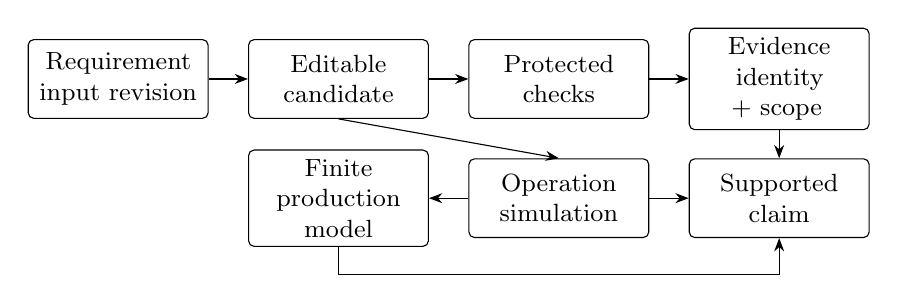
\begin{tikzpicture}[node distance=5mm and 5mm,box/.style={draw,rounded corners=2pt,align=center,font=\small,text width=2.05cm,minimum height=10mm},>={Stealth}]
\node[box] (req) {Requirement\\input revision};
\node[box,right=of req] (cand) {Editable\\candidate};
\node[box,right=of cand] (check) {Protected\\checks};
\node[box,right=of check] (store) {Evidence\\identity + scope};
\node[box,below=of check] (op) {Operation\\simulation};
\node[box,left=of op] (prod) {Finite production\\model};
\node[box,right=of op] (claim) {Supported\\claim};
\draw[->] (req)--(cand);\draw[->] (cand)--(check);\draw[->] (check)--(store);
\draw[->] (cand.south)--(op.north);\draw[->] (op)--(prod);\draw[->] (op)--(claim);
\draw[->] (store)--(claim);\draw[->] (prod.south)--++(0,-.35)-|(claim.south);
\end{tikzpicture}
\caption{Evidence flow at a shareable system abstraction. Candidate edits and protected evaluation have different authority. Geometry exports, operation simulation and production events are distinct representations. The production model consumes a qualified empirical operation envelope; it does not execute continuous multi-robot contact physics.}
\label{fig:architecture}
\end{figure}

\subsection{Outcome and freshness semantics}
\status{PASS} means the evaluated predicate passed within its stated scope. \status{FAIL} records an assessed violation. \status{UNKNOWN} records insufficient coverage or unresolved evidence. A runtime \status{CRASH} and a missing observation are operational failures, not geometric counterexamples; neither may silently become a pass. Stale and superseded observations remain available as historical records but cannot justify the current revision's status. The native interface exposes revision comparison, witnesses, repair traces and input freshness so that an earlier-input result is distinguishable from a current-input result.

Scope is particularly important for wall thickness. A short, verified in-material segment between appropriate surface supports can demonstrate an invalid wall. A finite set of samples cannot generally prove the global minimum exceeds a threshold. The revised feature checker therefore admits a local acceptance only for its declared feature and leaves whole-part acceptance unresolved. This is a deliberate limit of the result type, not a claim that every valid object can be certified.

\section{Study design}
The evidence combines newly executed checker, repair and gantry studies with previously collected fixture and production records. The supplement identifies each cohort and protocol separately. Their observations are never pooled across stages. All performance outcomes concern software checks or specified simulation models; no hardware or electrical measurement was collected.

\subsection{Checker truth and coverage}
The known-answer study contains 260 geometric cases and 100 additional nongeometry contract checks. Analytic constructions define truth independently of the checker under test. Four geometric assessments are compared: a sampled screen, a centerline witness, a feature-local checker and its whole-part projection. Global fixture truth governs the first, second and fourth assessments; feature-local truth governs the third when a feature exists. Error totals must therefore be read with the truth scope shown. Counts and runtime describe related parametric families, not independent manufactured parts.

\subsection{Budget-matched template repair}
Nine tasks form three families: arm sorting, arm seating and gantry timing. The arm families share a six-axis template; the gantry supplies the other underlying template. Each task has two sessions in each of three information conditions, giving 54 episodes and nine task clusters. All conditions receive common CAD and compile diagnostics. Aggregate feedback adds a protected development verdict. Structured witnesses add per-check detail and unit-bearing development measurements. The experimental agent is Codex CLI 0.162.1 using \texttt{gpt-6.1-sol} at medium reasoning effort. The service does not expose a reproducible sampling seed or model weights.

The arms share task definitions, starting designs and ceilings of four submitted revisions and 1,800 s per episode. The three arms of each task-session block run concurrently. The starting design is pre-evaluated symmetrically outside the episode timer and cannot be selected. Candidates change arm link dimensions and timing, or gantry timing alone; a trusted planner recomputes waypoints. The selected artifact is the last task-preserving, build-valid candidate with a completed receipt before closure. Selection never uses the hidden endpoint.

After a cohort seal, the selected and first build-valid candidates are scored on five held-out disturbance draws. Success requires all eligible geometry checks and all held-out operation checks to pass within the task window. \status{FAIL}, \status{UNKNOWN}, \status{CRASH} and missing candidates remain in the planned denominator. Development and hidden evaluation use the same evaluator family with different draws, so the hidden test controls draw reuse without establishing evaluator independence.

For task $t$, session $r$ and arm $a$, let $Y_{tra}$ denote selected-candidate success. The primary contrast is
\begin{equation}
 \widehat\Delta_{21}=\frac{1}{9}\sum_{t=1}^{9}
 \left(\frac{1}{2}\sum_{r=1}^{2}Y_{tr2}-\frac{1}{2}\sum_{r=1}^{2}Y_{tr1}\right).
\end{equation}
A fixed-seed percentile bootstrap resamples tasks, preserving the two sessions and arm pairing within each task. With nine related task clusters, its interval is descriptive and cannot establish equivalence. Provider token costs and starting-design work are reported separately from episode ceilings.

\subsection{Placement, speed and production}
The fixture intervention changes both the ring inner-edge chamfer from 0.4 to 3.0 mm and the key-slot entry flare from 0 to 3.0 mm. Previously collected held-out trials pair disturbance draws across original and revised geometry under fixed controller settings. The reference approach uses a 30 mm approach, 1.2 s insertion and 0.35 speed fraction; the secondary fast approach uses 8 mm, 0.2 s and 0.8. A selected independent replay tests one identified pair; it is not a rerun of the complete cohort.

The gantry experiment compares baseline and conic time profiles on the same geometric polyline, with unchanged simulated control authority. One hundred variant-pairs are grouped into 50 seed clusters. The complete-transfer endpoint and a prespecified $-0.10$ noninferiority margin are separate from planned path time. The clock excludes pre-settle and final hold.

The production study has original/revised fixtures crossed with FIFO/CP-SAT dispatch. Six fixed scenarios, 30 paired seeds and four cells produce 720 runs, or 180 paired quartets. A SimPy executor and an independent event checker assess runs; the planner has only information available at time zero. This model resamples a separate 40-pair fast-profile qualification envelope, not the primary 100-pair held-out fixture cohort.

\section{Results}
\subsection{Abstention preserves the distinction between local and global truth}
\begin{table}[tb]
\centering\small\begin{tabular}{llllllll}
\toprule
Checker & Truth & CA & CR & FA & FR & U & Crash \\
\midrule
Sampled screen & Global & 108 & 48 & 104 & 0 & 0 & 0 \\
Centerline witness & Global & 0 & 66 & 0 & 0 & 194 & 0 \\
Feature-local checker & Feature & 113 & 109 & 0 & 0 & 38 & 0 \\
Whole-part projection & Global & 0 & 109 & 0 & 0 & 151 & 0 \\
\bottomrule
\end{tabular}

\caption{Geometry outcomes over 260 cases. CA/CR: correct acceptance/rejection; FA/FR: false acceptance/rejection; U: abstention. Feature-local and global truth are different predicates. Counts do not establish equal-scope superiority of the local checker.}
\label{tab:checker}
\end{table}
The sampled screen accepted 104 globally invalid cases. The whole-part projection rejected 109 invalid cases, abstained on 151 cases and accepted none. The feature-local checker made 113 correct local acceptances and 109 correct rejections, with 38 abstentions and no observed errors under its own truth definition (Table~\ref{tab:checker}). These finite known-answer results support the stated scope; they are not universal wall-thickness certification.

The geometric failure mechanism is consequential: a sampling screen can miss thin material around screw-pilot features even when its summary appears acceptable. Reassessment of two archived bay frames and a pedestal found 0.51 mm walls below the unchanged 0.8 mm requirement, superseding three earlier passes. The prospective feature evaluator is not installed in the live production gate. Mean assessment time was 21.510 ms for the sampled screen, 2.295 ms for the centerline witness and 27.957 ms for the revised check, on the recorded pinned environment.

\subsection{Repairs occurred without an established richer-feedback effect}
\begin{table}[tb]
\centering\small\begin{tabular}{llllll}
\toprule
Feedback & $n$ & Pass & Fail & Other & Repairs \\
\midrule
CAD diagnostics & 18 & 14 & 4 & 0 & 0 \\
Aggregate feedback & 18 & 17 & 1 & 0 & 5 \\
Structured witnesses & 18 & 18 & 0 & 0 & 5 \\
\bottomrule
\end{tabular}

\caption{Selected-candidate held-out outcomes, including all planned episodes. Other includes unknown, crash and missing-candidate outcomes, all zero. Repairs count episodes whose first build-valid candidate fails and selected candidate passes. Each condition contains two sessions per task across nine tasks.}
\label{tab:repair}
\end{table}
Every episode completed without an unknown, crash or missing candidate. Selected-candidate passes were \EOneCadPass{}/18, \EOneAggregatePass{}/18 and \EOneStructuredPass{}/18 for CAD diagnostics, aggregate feedback and structured witnesses (Table~\ref{tab:repair}). The primary structured-minus-aggregate difference was \EOnePrimary{}, with task-cluster interval [0, \EOnePrimaryHigh{}]. The secondary aggregate-minus-CAD and structured-minus-CAD estimates were \EOneAggregateCad{} and \EOneStructuredCad{}; both intervals also include zero. These observations neither establish nor exclude a benefit from richer feedback.

\begin{figure}[tb]
\centering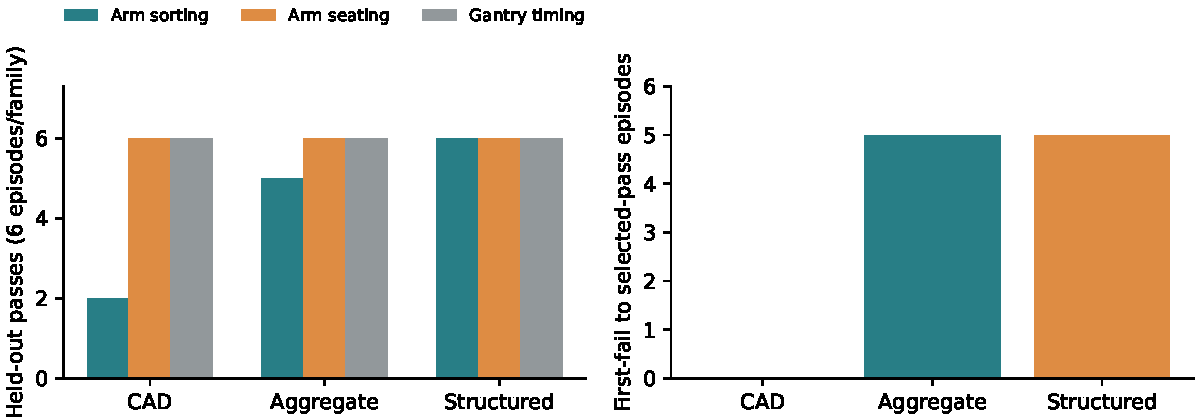
\includegraphics[width=\linewidth]{figures/repair_outcomes.pdf}
\caption{Family-specific success and completed successful repair. All arm-condition outcome differences occur in the sorting family; seating and gantry tasks pass in every episode. The right panel counts ten observed first-fail to selected-pass episodes, five under each protected-feedback condition. The small, shared-template task set limits generalization.}
\label{fig:repair}
\end{figure}

Ten episodes changed from an initially failing build-valid candidate to a passing selected candidate, five in each protected-feedback condition (Figure~\ref{fig:repair}). All between-condition outcome differences arose in three sorting tasks. The six seating and gantry task clusters passed in every condition. Timing-only tasks often admitted repairs inferable from the brief itself, limiting their ability to distinguish feedback mechanisms.

Transition accounting requires a separate qualification. The frozen protocol counted a changed selected ordinal of at least two relative to ordinal one. A pre-seal analysis implementation instead compared with the first build-valid candidate; this discrepancy was discovered after outcomes were visible. Literal counts are 3/6/6 across conditions, while build-valid-relative counts are 0/6/5. Neither definition means successful repair. The ten first-fail to selected-pass events provide the corresponding outcome evidence; the supplement reports both transition definitions.

Sessions ended voluntarily, with median wall durations near 100 s, below their 1,800 s ceilings. Reported input token totals increased from \TokensCad{} to \TokensAggregate{} and \TokensStructured{} across conditions. Equal revision and wall ceilings consequently do not establish equal total computation or equal cost. Continuous residuals also require caution: geometry checks are status-only components, so a geometry-failing candidate may have zero assessed continuous violation.

\subsection{A coupled fixture change improved the observed paired count}
\begin{table}[tb]
\centering\small\begin{tabular}{llll}
\toprule
Profile & Original & Revised & Original minus revised \\
\midrule
Reference approach & 96/100 & 100/100 & -0.040 \\
Fast approach & 91/100 & 98/100 & -0.070 \\
\bottomrule
\end{tabular}

\caption{Previously collected held-out simulated placement outcomes. Rows are separate controller profiles. The last column is original minus revised success proportion on shared draws; the coupled chamfer-and-flare intervention is not decomposable from these data.}
\label{tab:fixture}
\end{table}
Under the reference approach, \ETwoReferenceOriginal{}/100 original-fixture and \ETwoReferenceRevised{}/100 revised-fixture trials passed (Table~\ref{tab:fixture}), giving original-minus-revised $-0.040$. The secondary fast approach yielded \ETwoFastOriginal{}/100 and \ETwoFastRevised{}/100, or $-0.070$. A separate development example had 24/30 and 30/30; it is neither pooled with nor substituted for the held-out cohort. Per-cell Wilson intervals are descriptive and are not paired-effect intervals.

The engineering mechanism is a coupled capture-entry change. The larger chamfer and flared jaw entry can guide an offset housing into the unchanged throat, reducing the entry obstruction encountered by the original fixture. Because both features changed, the data do not identify either feature's isolated effect. The controller was held fixed within each profile, separating this comparison from a simultaneous control redesign.

One independently rerunnable pair reproduces archived trajectories and outcomes with identical library versions. Its original-fixture final yaw of approximately $3.4233^\circ$ exceeds a $3.3^\circ$ limit, while the revised case passes. Three exploratory $10^{-12}$ m position nudges changed the original decision to pass in two runs. This probe demonstrates sensitivity near the threshold; it does not estimate a flip probability. The four-count reference contrast must therefore remain conditional on the recorded contact model and numerical choices. Exported collision geometry also omits small regions present in the CAD model near the key-slot jaws, limiting physical interpretation of the visual mechanism.

\begin{figure}[p]
\centering
\textbf{(a) Coupled entry-geometry change}\par
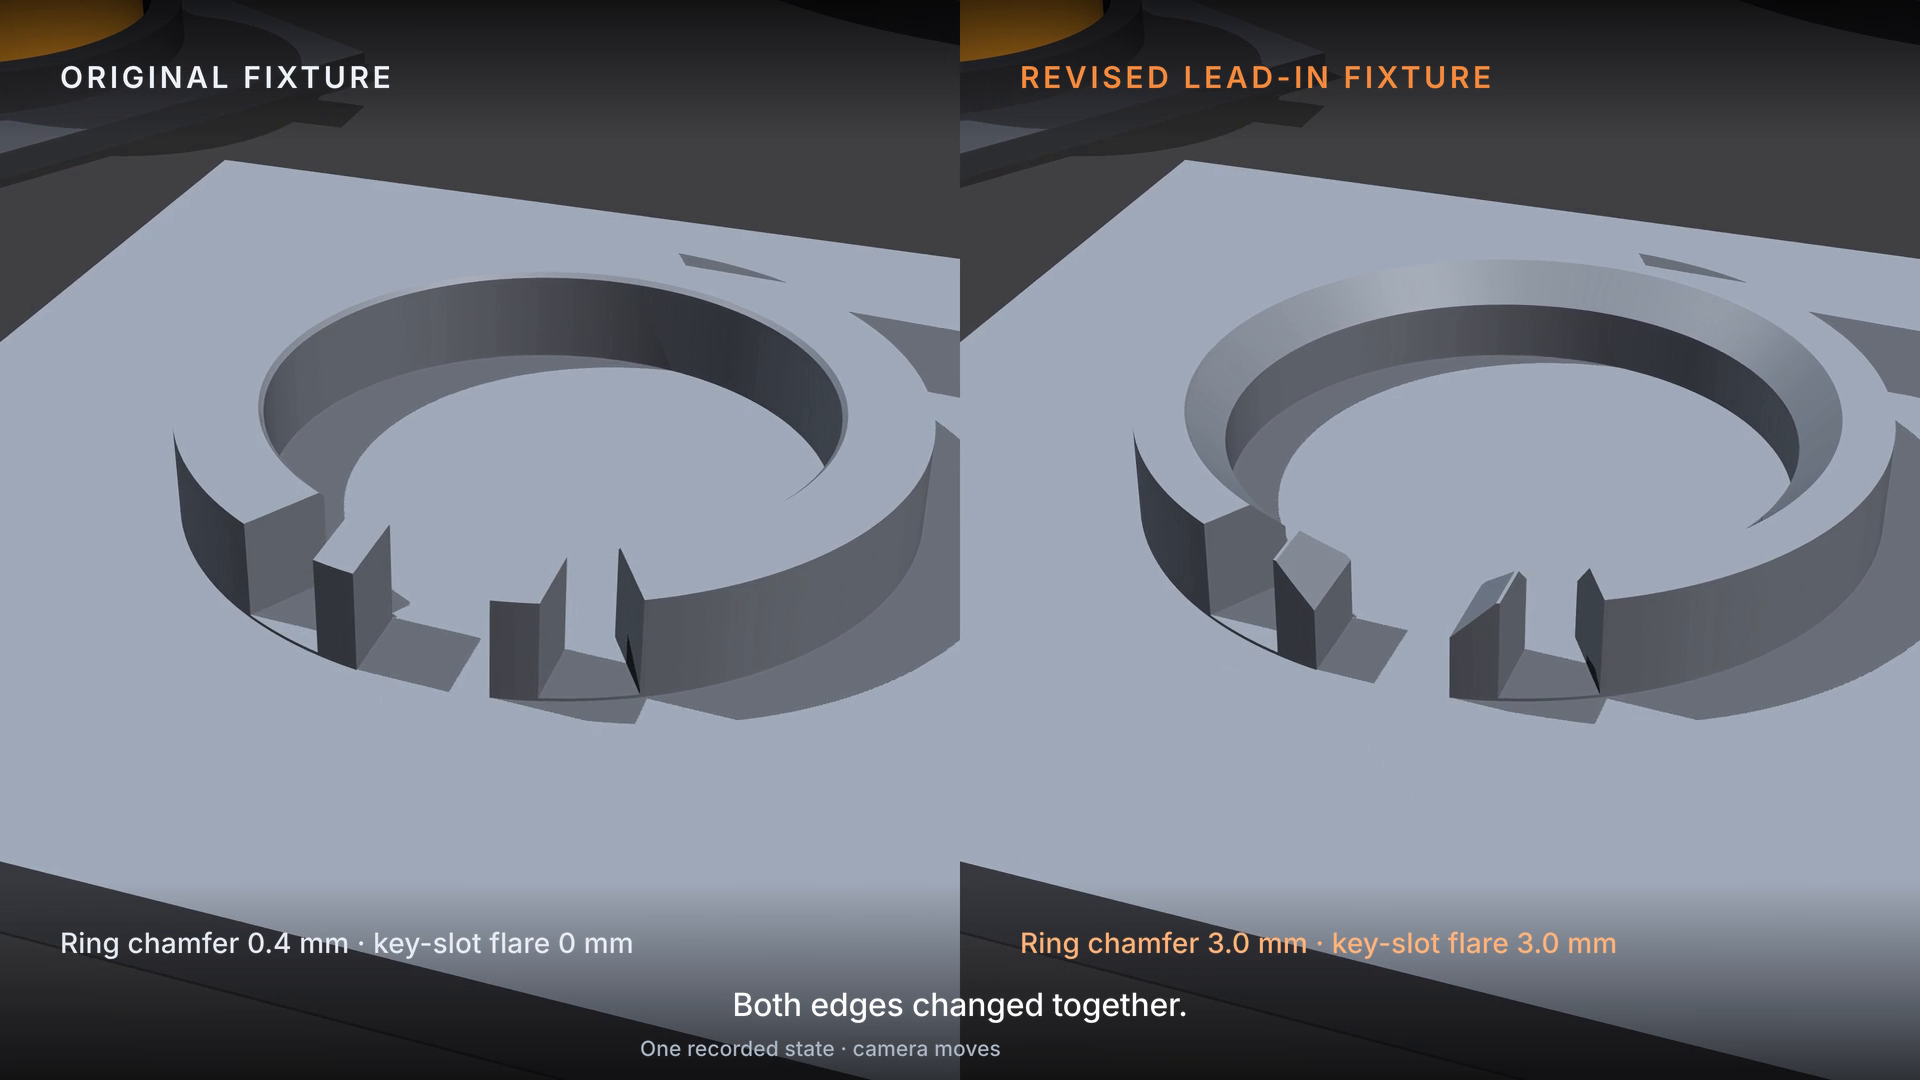
\includegraphics[width=.92\linewidth]{figures/fixture_geometry.png}\par
\textbf{(b) Final recorded poses in the representative paired trial}\par
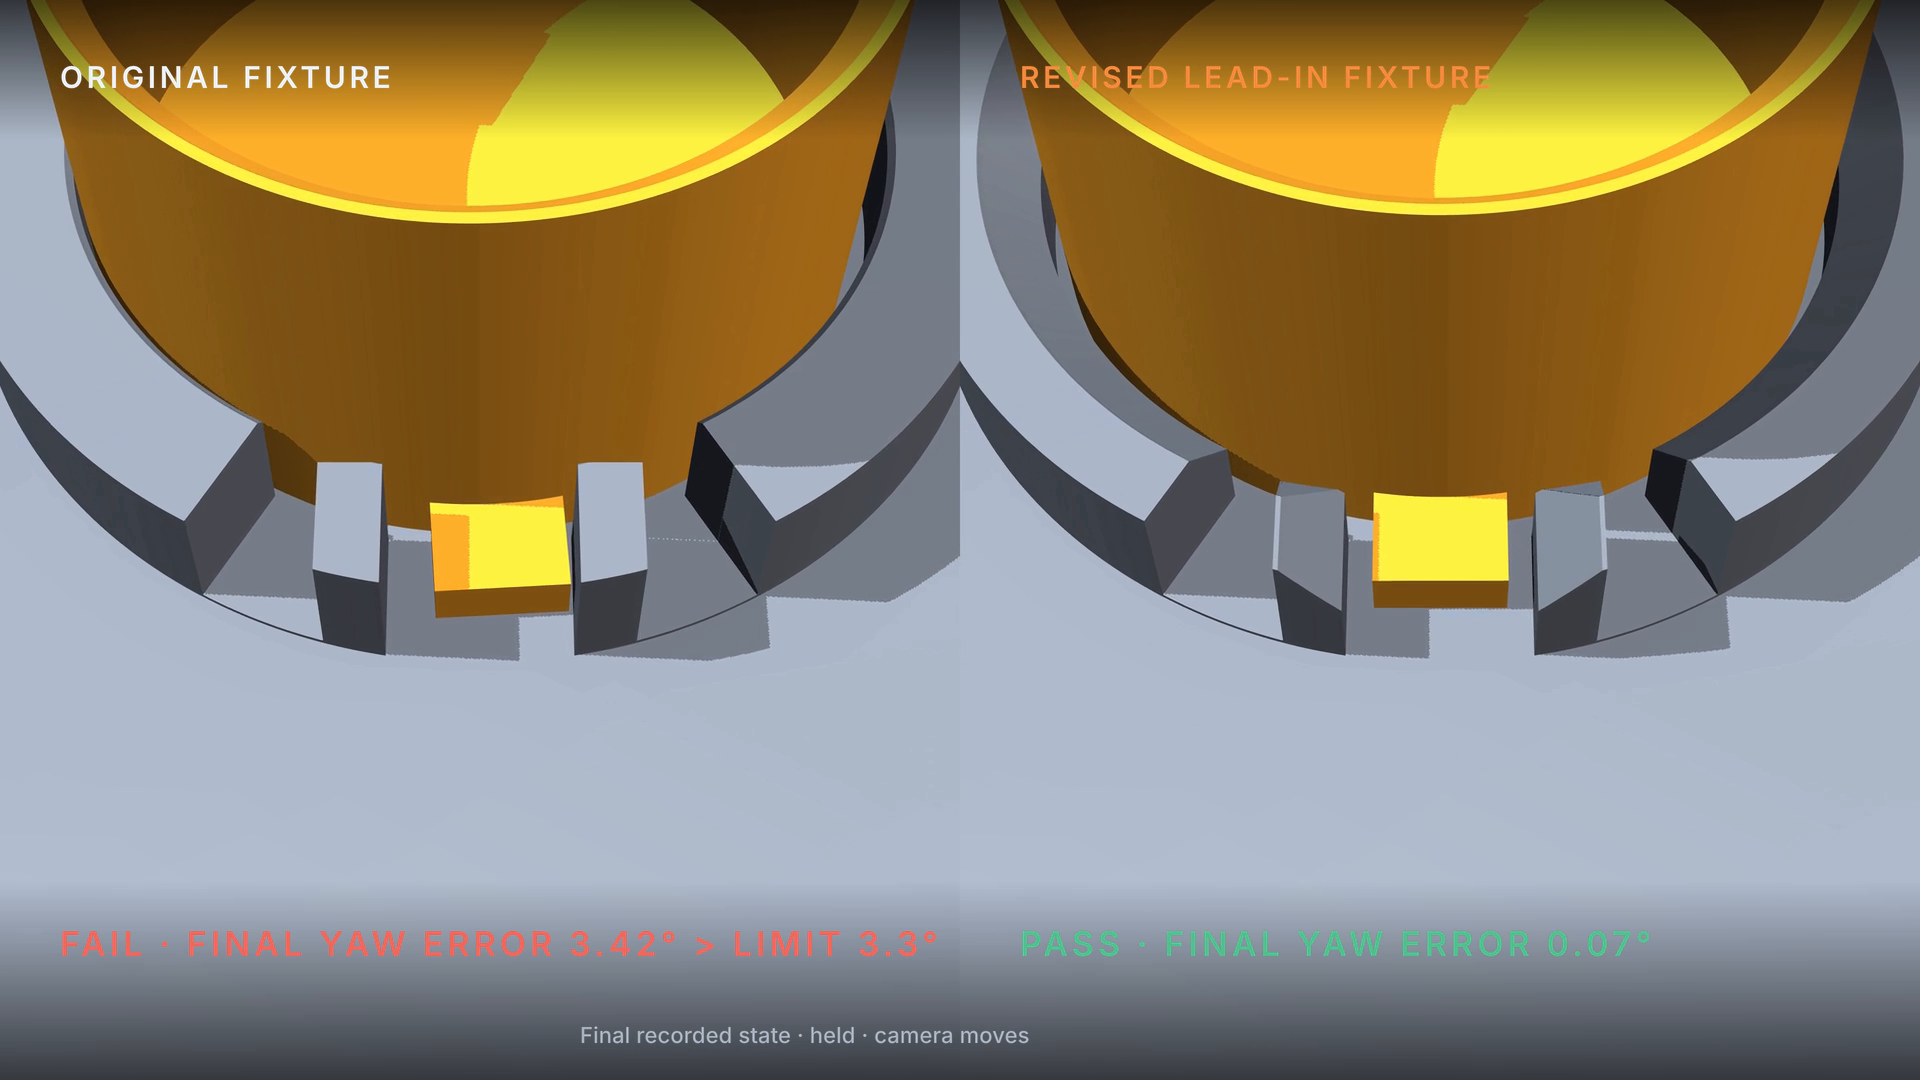
\includegraphics[width=.92\linewidth]{figures/fixture_contact.png}
\caption{Original and revised fixtures in verified visual copies of archived simulation geometry. (a) Both ring chamfer and slot flare change; isolated feature effects are not measured. (b) The prespecified representative pair uses the same disturbance and controller. Its original case fails the final yaw limit and its revised case passes. These are recorded simulated states, not hardware. Collision surfaces differ locally from complete CAD near the jaws.}
\label{fig:fixture}
\end{figure}

\begin{figure}[tb]
\centering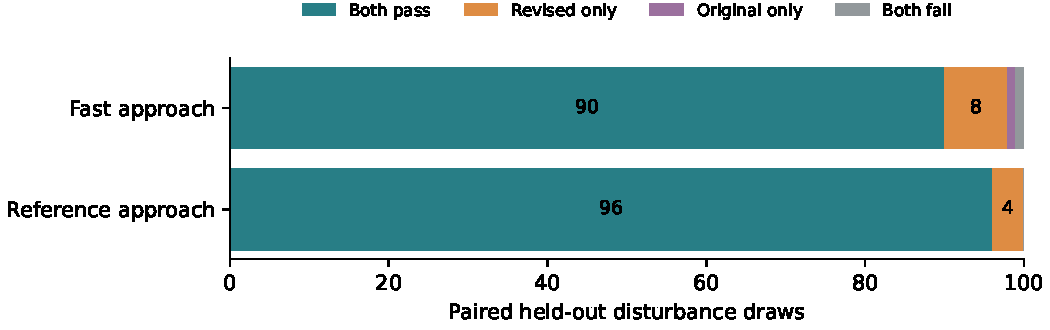
\includegraphics[width=\linewidth]{figures/paired_placements.pdf}
\caption{Joint outcomes on 100 shared held-out simulated draws per controller profile, preserving pairing between fixtures. Each bar partitions all draws into concordant and discordant outcomes. \PlacementPairSentence{} The profiles are distinct evaluations; neither bar includes the separate development cohort.}
\label{fig:paired}
\end{figure}

\section{Fixed-path speed optimization and transfer outcome}
\subsection{Modeled optimization problem}
For path coordinate $s$, define squared speed $b(s)=\dot s^2$ and path acceleration $a(s)=\ddot s$, giving $b'=2a$. Under a piecewise-linear squared-speed discretization, the implemented conic objective and dynamics are
\begin{align}
 \min_{b,a,e,d}\quad &\sum_i 2\Delta s_i d_i,\\
 b_{i+1}-b_i &= 2\Delta s_i a_i,\qquad
 e_j^2\le b_j,\qquad d_i(e_i+e_{i+1})\ge1.
\end{align}
Here $b,e,d$ are nonnegative, with speed caps, modeled torque bounds and rest conditions at endpoints and direction-changing corners. The supplement gives the actual torque and carried-tray constraints. The transformation follows established fixed-path speed optimization~\cite{lipp2014minimum}; it is feedforward time parameterization, not path planning or a new feedback controller.

The modeled drives are idealized position servos with speed-independent torque limits. Planning uses half of declared torque authority and 90\% of top speed, with conservative inertia, damping and friction margins. Carried segments enforce a non-slip acceleration constraint and a downward-acceleration bound. Baseline motion stops at every segment; the optimized profile passes through a collinear lowering boundary. The geometric path is shared, while its rest pattern changes by design.

\subsection{A faster plan left docking unresolved}
\begin{table}[tb]
\centering\small\begin{tabular}{llllll}
\toprule
Profile & Pass & $n$ & Planned s & Unseated & Work J \\
\midrule
baseline & 59 & 100 & 21.760 & 40 & 3.147 \\
optimised & 58 & 100 & 7.474 & 40 & 5.331 \\
\bottomrule
\end{tabular}

\caption{Gantry outcomes on 100 paired simulated draws per profile. Planned duration excludes 0.6 s pre-settle and 1.0 s hold. Work denotes simulated mechanical work, not electrical energy. Unseated counts remain in the success denominator.}
\label{tab:gantry}
\end{table}
The used profile has planned duration \GantryOptimisedPrecise{} s, compared with \GantryBaselineTime{} s for the baseline (Table~\ref{tab:gantry}). Successful transfers changed from \GantryBaselinePass{}/100 to \GantryOptimisedPass{}/100. The paired optimized-minus-baseline difference is $\GantryDifference{}$, with seed-cluster interval $[\GantryLow{},\GantryHigh{}]$, satisfying the frozen $-0.10$ noninferiority rule but providing no evidence of improved reliability. Both profiles leave the tray unseated in 40/100 runs. Their failure exposes a docking/capture problem that retiming does not resolve.

The numerical optimum has a limited meaning. An exact solution of the same bounded continuous model gives \GantryContinuous{} s; the discretized feasible set restricts that model, so a numerically feasible discrete solution gives an upper bound on that modeled optimum. The reported solver iterate requires its separate feasibility checks. A speed-only relaxation gives a model-specific lower bound. Neither direction certifies a physical gantry's achievable transfer time. Raw solver residuals exceed the requested $10^{-8}$ tolerance in some constraints, and an 800-grid refinement includes an inaccurate solver status; detailed feasibility checks belong alongside the objective value. Simulated completion, physical actuator behavior and reliable docking remain separate requirements.

\section{Conditional production effects}
The model uses OR-Tools 9.15.6755 for CP-SAT and SimPy 4.1.2 for discrete-event execution~\cite{cpsatlp,simpy412}.
Let $G_{ms}$ denote good units for mechanical condition $m$ and dispatch condition $s$, with zero indexing original geometry or FIFO. The reference-cell contrasts are
\begin{align}
 D_M&=G_{10}-G_{00},&D_S&=G_{01}-G_{00},\\
 D_C&=G_{11}-G_{00},&D_I&=G_{11}-G_{10}-G_{01}+G_{00}.
\end{align}
These are reference-cell contrasts, not mechanically averaged factorial main effects. Their six-scenario means are \EThreeMechanical{}, \EThreeScheduling{}, \EThreeCombined{} and \EThreeInteraction{} good units per modeled run, respectively. Dispatch contributes more than the mechanical-only contrast. The combined contrast equals the sum of the two reference-cell contrasts and their interaction.

\begin{figure}[tb]
\centering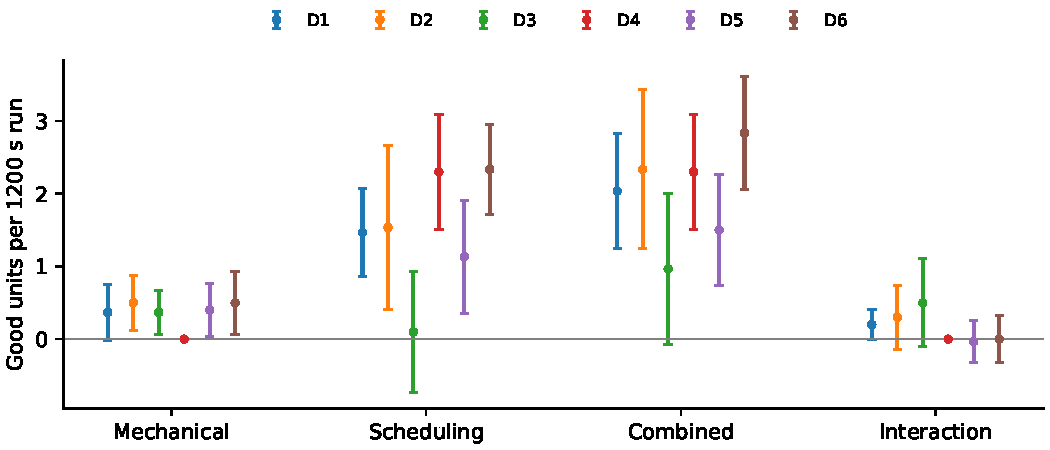
\includegraphics[width=\linewidth]{figures/production_contrasts.pdf}
\caption{Scenario-specific mean contrasts over 30 paired production seeds each, with conditional paired t intervals. Colors identify six fixed scenarios, not a sampled factory population. The operation envelope is held fixed; variation across production seeds excludes uncertainty in its estimation and in the contact model. Complete four-cell tables are in the supplement.}
\label{fig:production}
\end{figure}

The model evaluates 40 orders over a 1,200 s horizon. CP-SAT plans with qualified mean times, a window of eight and only orders known at time zero; the SimPy executor generates the assessed event traces. All 720 runs have passing independent event checks. A valid trace establishes consistency with the event contract, not the validity of its operation-time distribution. These calculations show how a specified empirical operation envelope affects a finite planning model. They do not predict a population of factories or supply continuously coupled multi-robot physics.

\section{Discussion, limitations and reproduction}
The results make evidence scope operational. Local geometry acceptance can coexist with global abstention; a changed candidate is not necessarily a repaired task; a shorter planned trajectory can coexist with unresolved transfer failures; a mechanically improved operation need not dominate downstream scheduling gains. The system preserves these distinctions through evaluation identity and outcome semantics. They would be lost if every artifact were reduced to a single success badge.

The feedback study now contains real candidate-to-candidate repairs, while the archived 54-episode study contained none and substantial worker crashes. Changes to the execution harness make the newer study interpretable; they do not create a causal feedback comparison against the earlier cohort. The new randomized block ordering and sealed scoring support the within-cohort comparison only. Shared templates, nine task clusters, service-dependent generation and an easily inferred timing repair limit external validity.

Native product journeys exercised three briefs and six revisions, all still \status{NOT\_READY}. Their receipts support implemented navigation, revision comparison and stale-input behavior in isolated runtimes. Operator-staged edits make them demonstrations rather than an autonomy benchmark. The tested changes are not installed in the owner's live production application. A complex quadruped visualization, when shown, belongs to a separate identified design under test and contributes no samples to the fixture or repair studies.

The study artifact supports offline verification, arithmetic, analysis tests and regenerated figures without Forge (Tier A). A data-only MuJoCo replay supports one selected fixture pair (selected Tier B). It does not independently reproduce all placement trials, the production engine or provider sessions. Proprietary orchestration and prompt-to-design execution are unavailable at Tier C. The supplement specifies pinned environments, exact commands and data dictionaries. The accompanying artifact is limited to shareable evidence; no DOI has been assigned to the study.

No physical robot, factory, certification or electrical-energy measurement is established. Contact approximations, numerical decision sensitivity, idealized actuators, finite task selection and fixed production scenarios constrain interpretation. The evidence supports bounded software and model conclusions, including negative findings. It does not turn an accepted model or an optimal plan into physical readiness.

\section{Conclusion}
Forge links editable robot revisions to scoped checks, conditional operation trials and a separately evaluated production model. The studies demonstrate completed design repairs, a coupled fixture comparison and a conic retiming application, while leaving richer-feedback efficacy, physical reliability and gantry docking unresolved. The central engineering result is an inspectable chain in which each conclusion retains its predicate, revision and evaluation context, including where the chain stops short of a complete task.
\bibliographystyle{plainnat}
\bibliography{references}
\end{document}
